\documentclass[11pt]{article}
\usepackage[utf8]{inputenc} % Para caracteres en espa�ol
\usepackage{amsmath,amsthm,amsfonts,amssymb,amscd}
\usepackage{multirow,booktabs}
\usepackage[table]{xcolor}
\usepackage{fullpage}
\usepackage{lastpage}
\usepackage{enumitem}
\usepackage{multicol}
\usepackage{fancyhdr}
\usepackage{mathrsfs}
\usepackage{pdfpages}
\usepackage{wrapfig}
\usepackage{setspace}
\usepackage{esvect}
\usepackage{calc}
\usepackage{multicol}
\usepackage{cancel}
\usepackage{graphicx}
\graphicspath{ {pictures/} }
\usepackage[retainorgcmds]{IEEEtrantools}
\usepackage[margin=3cm]{geometry}
\usepackage{amsmath}
\newlength{\tabcont}
\setlength{\parindent}{0.0in}
\setlength{\parskip}{0.05in}
\usepackage{empheq}
\usepackage{framed}
\usepackage[most]{tcolorbox}
\usepackage{xcolor}
\colorlet{shadecolor}{orange!15}
\parindent 0in
\parskip 12pt
\geometry{margin=1in, headsep=0.25in}
\theoremstyle{definition}
\newtheorem{defn}{Definition}
\newtheorem{reg}{Rule}
\newtheorem{exer}{Exercise}
% Two more packages that make it easy to show MATLAB code
\usepackage[T1]{fontenc}
\usepackage[framed,numbered]{matlab-prettifier}
\lstset{
	style = Matlab-editor,
	basicstyle=\mlttfamily\small,
}
\newtheorem{note}{Note}
\begin{document}  
\setcounter{section}{0}
\thispagestyle{empty}

\begin{center}
{\LARGE \bf Homework 4}\\
{\large AE370 - Spring 2018 \\ Emilio R. Gordon}
\end{center}
\vspace{0mm}
\textbf{Problem: Steady-state fluid problem} \\
Use the finite difference method to solve the following incompressible/inviscid fluid flow problem:\\
%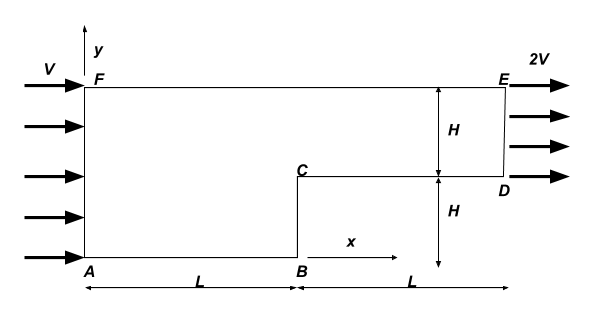
\includegraphics[scale=0.7]{1.png}\\
\noindent\makebox[\textwidth]{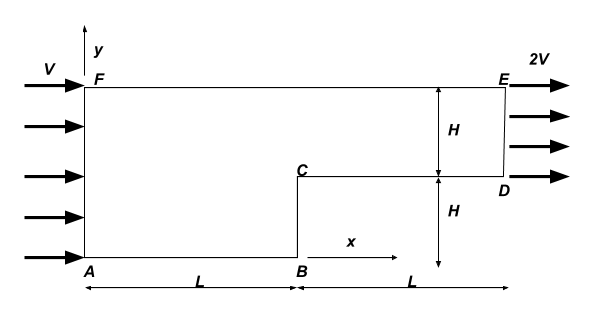
\includegraphics[scale=0.8]{1.png}}
The flow problem can be described by the following GDE:
\begin{equation*}
\begin{aligned}
\frac{\partial^2 \Phi}{\partial x^2}+\frac{\partial^2 \Phi}{\partial y^2} = 0
\end{aligned}
\end{equation*}
where the streamline function $\Phi$ is related to the x and y components of the velocity vector through:
\begin{equation*}
\begin{aligned}
V_x = \frac{\partial \Phi}{\partial y} \qquad V_y = -\frac{\partial \Phi}{\partial x}
\end{aligned}
\end{equation*}
The boundary conditions are:
\begin{equation*}
\begin{aligned}
\Phi &= V_y &\qquad \text{along AF}\\
\Phi &=2VH &\qquad \text{along FE}\\
\Phi &=2V(y-H) &\qquad \text{along DE}\\
\Phi &=0 &\qquad \text{along ABCD}\\
\end{aligned}
\end{equation*}
\newpage
Use a second-order central diffrence scheme to solve the problem using N, grid spacings to discretize L (i.e. $\Delta x = L/N_x$) and $N_y$ grid spacings to discretize H (i.e., $\Delta y = H/N_y$).
\begin{enumerate}[label=(\alph*)]
\item Derive the discretized form of the PDE
\item Choose a numbering of the grid points (Describe it thoroughly in your report!) and put together the matrix equation.
\item Implement the boundary conditions.
\item Write a Matlab code that solves this problem. As output you should create the following three plots:
\begin{enumerate}
\item A contour plot for the streamline function (using the command \texttt{CONTOUR})
\item A vector plot for the velocity field (using the central difference approximation for the first derivatives of the streamline function and the command \texttt{QUIVER})
\item A x-y plot of the pressure distribution along the edge boundary condition, where the pressure is obtained by $P = \rho (V_x^2 + V_y^2)$ where $\rho$ is the fluid density.
\end{enumerate}
\item Solve the problem for L=1 [m], H = 0.2 [m], V = 1 [m/s] and $\rho=1 [kg/m^3]$. Perform a convergence study to determine the appropriate values of $N_x$ and $N_y$. Comment on your solution and especially on the computed solution in the vicinity of the corner.
\end{enumerate}


\textbf{Solution:} 
\end{document}